\documentclass{beamer}
\setbeamertemplate{navigation symbols}{}
\usepackage[justification=centering]{caption}

\usepackage{amsmath}
% \usetheme{Warsaw}
%\usetheme{default}
%\usetheme{AnnArbor}
%\usetheme{Antibes}
%\usetheme{Bergen}
%\usetheme{Berkeley}
%\usetheme{Berlin}
%\usetheme{Boadilla}
%\usetheme{CambridgeUS}
%\usetheme{Copenhagen}
%\usetheme{Darmstadt}
%\usetheme{Dresden}
%\usetheme{Frankfurt}
%\usetheme{Goettingen}
%\usetheme{Hannover}
%\usetheme{Ilmenau}
%\usetheme{JuanLesPins}
%\usetheme{Luebeck}
%\usetheme{Madrid}
\usetheme{Malmoe}
%\usetheme{Marburg}
%\usetheme{Montpellier}
%\usetheme{PaloAlto}
%\usetheme{Pittsburgh}
%\usetheme{Rochester}
%\usetheme{Singapore}
%\usetheme{Szeged}
%\usetheme{Warsaw}

% As well as themes, the Beamer class has a number of color themes
% for any slide theme. Uncomment each of these in turn to see how it
% changes the colors of your current slide theme.

%\usecolortheme{albatross}
%\usecolortheme{beaver}
%\usecolortheme{beetle}
%\usecolortheme{crane}
%\usecolortheme{dolphin}
%\usecolortheme{dove}
%\usecolortheme{fly}
%\usecolortheme{lily}
%\usecolortheme{orchid}
%\usecolortheme{rose}
%\usecolortheme{seagull}
%\usecolortheme{seahorse}
%\usecolortheme{whale}
%\usecolortheme{wolverine}
\usepackage{biblatex}
%\usepackage{url}
%\usepackage{cite}

\beamersetuncovermixins{\opaqueness<1>{25}}{\opaqueness<2->{1}}

\begin{document}
\title{Application of Wavelet in Computer Graphics: Wavelet Radiosity}  
\author{Pinkesh Barsopia (123079006) }
\institute{Guide: Prof. V. M. Gadre \\ Department of Electrical Engineering \\ Indian Institute of Technology Bombay}
\date{May 26, 2015}


\begin{frame}
\titlepage
\end{frame}
\begin{frame}[shrink]\frametitle{Outline}
\tableofcontents
\end{frame} 


\section{Introduction} 

  \subsection{Image Synthesis in Computer Graphics}

      \begin{frame}\frametitle{Direct and Indirect Illumination}
      \begin{itemize}
      \setlength\itemsep{1.5 em}
      \item Rendering-Image synthesis from closed scene given
      \begin{itemize}
      \item Geometry of scene
      \item Optical properties of surfaces (BRDF)
      \item Location of Light Source
      \end{itemize}
      \item Types of renderer
      \begin{itemize}
      \setlength\itemsep{0.5 em}
      \item Direct illumination
      \item Indirect Illumination (Global Illumination)
      \end{itemize}
      \item Types of Indirect Illumination renderer
      \begin{itemize}
      \setlength\itemsep{0.5 em}
      \item Ray-Tracing
      \item Radiosity (Lambertian BRDF)
      \end{itemize}
      \end{itemize}
      \end{frame}



      \begin{frame}\frametitle{Direct and Indirect Illumination}
       \begin{figure}
        \centering
        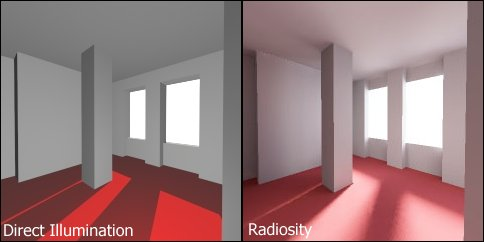
\includegraphics[width=4in]{DirectIndirect.jpg}
        \caption{Direct and Indirect Illumination\footfullcite{www.wikipedia.org/wiki/Radiosity(computer graphics)}}
        \label{idealscalable}
        \end{figure}
      \end{frame}



  \subsection{Radiosity Integral Equation (RIE)}


      \begin{frame}\frametitle{Radiosity Integral Equation (RIE)}

      Radiosity $\rightarrow $ Power (light) per unit area
      
      \begin{equation}
      B_i=E_i+\sum_j K_{i,j} B_j, \quad j \in \{All surfaces\}
      \end{equation}
      
      \centering
      $K_{i,j}=\frac{\text {Radiosity received by i from j}}{\text{Radiosity leaving from j}}$\\
      
      \vspace{2 mm}
      \centering
      $E_i \rightarrow $  Non zero for light source\\
      
      \vspace{2 mm}
      \centering
      $p_i \rightarrow $  BRDF of surface i\\

      \vspace{2 mm}
      \centering
      Domain of surfaces $(M^2) is L^2(\mathbb{R}^2)$ with finite support

      \begin{equation}
      B(x)=E(x)+p(x)\int_{M^2} K(x,y)B(y)\quad  \forall x \in M^2
      \end{equation}
      \end{frame}


\section{Literature Survey}

      \begin{frame}\frametitle{Literature Survey}

      \begin{itemize}
      \item Cohen et al. solved with $n$ patches (constant radiosity) and $n^2$ from factors, $K_{i,j}, \quad i,j =1,2,...,n.$

      \item Kajia $\rightarrow$ radiosity integral equation $\rightarrow$ Projection methods (solve RIE in finite space).

      \item Finite space
          \begin{itemize}
          \item Heckbert $\rightarrow$ Piecewise linear 
          \item Zatz $\rightarrow$ Piecewise polynomial of higher order
          \item Hanarahan et al. $\rightarrow$ Hierarchy of basis (Haar wavelet basis)
          \end{itemize}

      \item Gortler et al. $\rightarrow$ used wavelet basis $\rightarrow$ wavelet radiosity

      \end{itemize}
      \end{frame}


\section{Test Scenes and Metric for Comparison}
  \subsection{Radiosity in 2 and 3 Dimensions}


       \begin{frame}\frametitle{Test Scenes: 3 Dimensional}
       \vspace{-0.5 cm}
          \begin{columns}[T]
            \begin{column}{.4\textwidth}
        
    % Your text here
                \begin{figure}
                \centering
                \includegraphics[width=2 in]{3dparallel.png}
                \centering
                \caption{3D scene: Two parallel surfaces}
                \label{fig_parallel_3D}
                \end{figure}
                

            \end{column}
          \begin{column}{.5\textwidth}

                \begin{figure}
                \centering
                \includegraphics[width=2 in]{xy.png}
                \caption{3D Geometry: Kernel calculation}
                \label{fig_xy}
                \end{figure}
          \end{column}
        \end{columns}

          \begin{equation} \label{eq:3dkernel}
          K(x,y) =  \frac{\cos \theta_x \cos \theta_y} {\pi r_{xy}^{2}} V(x,y) 
          \end{equation}
          
     
        \end{frame}


  % \subsection{}

      \begin{frame}\frametitle{Test Scenes: 2 Dimensional}
        \begin{columns}[T]
          \begin{column}{.4\textwidth}
      
                \begin{figure}
              \centering
              \captionsetup{justification=centering}

              \includegraphics[width=1.2in]{f1_025.png}
              \caption{Flatland scene 1: parallel segments}
              \label{fig_parallel}
              \end{figure}
                  

          \end{column}
        \begin{column}{.5\textwidth}

                   \begin{figure}
                \centering
              \captionsetup{justification=centering}

                \includegraphics[width=2in]{f2.png}
                \caption{Flatland scene 2: perpendicular segments}
                \label{fig_parallel}
                \end{figure}
        \end{column}
      \end{columns}
    \end{frame} 





    \begin{frame}\frametitle{Kernel Calculation: 2 Dimensional }

          \begin{figure}
          \centering
          \includegraphics[width=1.8in]{kernel.png}
          \caption{ In general, kernel for two line segments X,Y}
          \label{fig_gen_kernel_2D}
          \end{figure}

          \vspace{-5 mm}

          \begin{equation} \label{eq:2dkernel}
          K(x,y) =  \frac{\cos \theta_x \cos \theta_y} {2 r_{xy}}V(x,y) 
          \end{equation}

    \end{frame}


    \begin{frame}\frametitle{Solution of Flatland Scenes 1}
    \vspace{-7 mm}
        
        \begin{columns}[T]
          \begin{column}{.4\textwidth}
      
              \begin{figure}
              \centering
              \includegraphics[width=1.8in]{f1_025_qlmw_scale_b1_plot_n_64.png}
              \caption{Radiosity $B_1(x)$}
              \label{fig_gen_kernel_2D}
              \end{figure}
        \end{column}

        \begin{column}{.5\textwidth}
              \begin{figure}
              \centering
              \includegraphics[width=1.8in]{f1_025_qlmw_scale_b2_plot_n_64.png}
              \caption{Radiosity $B_2(y)$}
              \label{fig_gen_kernel_2D}
              \end{figure}
        \end{column}
      \end{columns}
        \begin{columns}[T]
          \begin{column}{.4\textwidth}
      
              \begin{figure}
              \centering
              \includegraphics[width=1.5in]{qlmw_scale_64_025_b1.png}
              \caption{Image of $B_1$}
              \label{fig_gen_kernel_2D}
              \end{figure}
        \end{column}

        \begin{column}{.5\textwidth}

                \begin{figure}
              \centering
              \includegraphics[width=1.5in]{qlmw_scale_64_025_b2.png}
              \caption{Image of $B_2$}
              \label{fig_gen_kernel_2D}
              \end{figure}
        \end{column}
      \end{columns}


    \end{frame}

\begin{frame}\frametitle{Solution of Flatland Scenes 2}
    \vspace{-7 mm}
      \begin{columns}[T]
          \begin{column}{.4\textwidth}
      
              \begin{figure}
              \centering
              \includegraphics[width=1.8in]{f2_qlmw_scale_b1_plot_n_64.png}
              \caption{Image of $B_1$}
              \label{fig_gen_kernel_2D}
              \end{figure}
        \end{column}

        \begin{column}{.5\textwidth}

                \begin{figure}
              \centering
              \includegraphics[width=1.8in]{f2_qlmw_scale_b2_plot_n_64.png}
              \caption{Image of $B_2$}
              \label{fig_gen_kernel_2D}
              \end{figure}
        \end{column}
      \end{columns}
        \begin{columns}[T]
          \begin{column}{.5\textwidth}
      
              \begin{figure}
              \centering
              \includegraphics[width=1.5in]{f2_qlmw_scale_64_025_b1.png}
              \caption{Radiosity $B_1(x)$}
              \label{fig_gen_kernel_2D}
              \end{figure}
        \end{column}

        \begin{column}{.5\textwidth}
              \begin{figure}
              \centering
              \includegraphics[width=1.5in]{f2_qlmw_scale_64_025_b2.png}
              \caption{Radiosity $B_2(y)$}
              \label{fig_gen_kernel_2D}
              \end{figure}
        \end{column}
      \end{columns}
    \end{frame}



% \begin{frame}\frametitle{Solution of Flatland scenes 2}
%   \begin{figure}
%   \centering
%   \includegraphics[width=0.5in]{f2_qlmw_scale_64_025_b1.png}
%   \caption{General kernel for two line segments}
%   \label{fig_gen_kernel_2D}
%   \end{figure}
%     \begin{figure}
%   \centering
%   \includegraphics[width=0.5in]{f2_qlmw_scale_64_025_b2.png}
%   \caption{General kernel for two line segments}
%   \label{fig_gen_kernel_2D}
%   \end{figure}
%     \begin{figure}
%   \centering
%   \includegraphics[width=0.5in]{f2_qlmw_scale_b1_plot_n_64.png}
%   \caption{General kernel for two line segments}
%   \label{fig_gen_kernel_2D}
%   \end{figure}
%     \begin{figure}
%   \centering
%   \includegraphics[width=0.5in]{f2_qlmw_scale_b2_plot_n_64.png}
%   \caption{General kernel for two line segments}
%   \label{fig_gen_kernel_2D}
%   \end{figure}

% \end{frame}


  \subsection{Relative Error}

    \begin{frame}\frametitle{Metric for Comparison}
        
        Relative error($L^2$ norm) in K for comparison
        
        \begin{equation}
        \text{relative  error}=\frac{\int\int \,(\,K(x,y)-\hat{K}(x,y)\,)^2  \,dy \, dx}{\int\int \,K(x,y)^2  \,dy \, dx}
        \end{equation}
        
        Relative error ($L^2$ norm)  in B for comparison
        
        \begin{equation}
        \text{relative  error}=\frac{\int \,(\,B(x)-\hat{B}(x)\,)^2  \,dx}{\int \,B(x)^2  \,dx}
        \end{equation}
    \end{frame}



\section{Projection Methods for Radiosity}

    \begin{frame}\frametitle{Projection Methods for Radiosity}

    \end{frame}








\subsection{Choice of a Finite Space}
    \begin{frame}\frametitle{Choice of a Finite space}
        
      Space of Piecewise polynomial function of order m, over standard interval ($\frac{1}{n}$)
      \begin{columns}[T]
         \begin{column}{.5\textwidth}
      
            \begin{figure}
            \centering
            \includegraphics[width=1in]{f1_025_error_vs_n_all_three.png}
            \caption{Error in projection of K(x,y) for Flatland scene 1}
            \label{fig_e_vs_n_f1}
            \end{figure}
        \end{column}
         \begin{column}{.5\textwidth}

            \begin{figure}
            \centering
            \includegraphics[width=1in]{f2_025_error_vs_n_all_three.png}
            \caption{Error in projection of K(x,y) for Flatland scene 2}
            \label{fig_e_vs_n_f2}
            \end{figure}
        \end{column}
        \end{columns}
\end{frame}




\begin{frame}\frametitle{Analytical Solution}
\begin{equation}
  B(x)=1+\int K(x,y)B(y)dy
\end{equation}
\centering
$  K(x,y)=x^2+xy, \quad x,y \in [0,1]$\\
\centering
Degenerate kernel, $K(x,y) = \sum\limits_{i=1}^na_i(x)b_i(y) $
 
      \begin{columns}[T]
         \begin{column}{.5\textwidth}

              \begin{figure}
              \centering
              \includegraphics[width=1.5 in]{ahaar4.png}
              \caption{Solution using\\ $n=4,m=0$}
              \label{fig_e_vs_n_f1}
              \end{figure}
        \end{column}
         \begin{column}{.5\textwidth}

              \begin{figure}
              \centering
              \includegraphics[width=1.5 in]{ahaar16.png}
              \caption{Solution using $n=16,m=0$}
              \label{fig_e_vs_n_f2}
              \end{figure}
        \end{column}
        \end{columns}
\end{frame}



    \begin{frame}\frametitle{Analytical Solution for $m=1,2$}
    \vspace{-7 mm}
      \begin{columns}[T]
        \begin{column}{.5\textwidth}
      
    % Your text here
              \begin{figure}
              \centering
              \includegraphics[width=1.5in]{allmw2.png}
              \caption{Solution using $n=2,m=1$}
              \label{fig_e_vs_n_f1}
              \end{figure}

        \end{column}
      \begin{column}{.5\textwidth}

              \begin{figure}
              \centering
              \includegraphics[width=1.5in]{allmw4.png}
              \caption{Solution using $n=4,m=1$}
              \label{fig_e_vs_n_f2}
              \end{figure}

      \end{column}
    \end{columns}

    \vspace{-6 mm}

    \begin{columns}[T]
      \begin{column}{.5\textwidth}
      
              % Your text here
              \begin{figure}
              \centering
              \includegraphics[width=1.5in]{aqlmw1.png}
              \caption{Solution using $n=1,m=2$}
              \label{fig_e_vs_n_f1}
              \end{figure}

      \end{column}
      \begin{column}{.5\textwidth}
              \begin{figure}
              \centering
              \includegraphics[width=1.5in]{aqlmw2.png}
              \caption{Solution using $n=2,m=2$}
              \label{fig_e_vs_n_f2}
              \end{figure}

        \end{column}
      \end{columns}
    \end{frame}


  \subsection{Choice of a Basis}

    \begin{frame}
    \frametitle{Choice of a Basis: Wavelets}
    Choice of alternative basis for chosen space
        \begin{itemize}
        \item Haar
        \item Linear Legendre Multi-Wavelet
        \item Quadratic Legendre Multi-Wavelet
        \end{itemize}

     Advantages
        \begin{itemize}
        \item Vanishing Moments
        \item Negligible coefficients
        \item Sparse System of equation
        \item Faster Solution
        \end{itemize}
    \end{frame}

% \\section{choice of basis} % (fold)
% \label{sec:choice_of_basis}

% % section choice_of_basis (end)
    \begin{frame}
    \frametitle{Haar Wavelet: Alternate Basis}

        \vspace{-0.5cm}
        Haar Wavelet
        \vspace{-0.5cm}

          \begin{columns}[T]
            \begin{column}{.5\textwidth}

                \begin{equation}\label{eq:qlmwphi0}
                \phi(x)=
                \left\{
                    \begin{array}{ll}
                        1  and \mbox{if } 0 \leq x < 1 \\
                        0 and elsewhere
                    \end{array}
                \right.
                \nonumber
                \end{equation}

        \end{column}
        \begin{column}{.5\textwidth}

              \begin{equation}
              \psi^0(x)=
              \left\{
                  \begin{array}{ll}
                      1 and \mbox{if } 0 \leq x < \frac{1}{2} \\
                      -1  and \mbox{if } \frac{1}{2} \leq x < 1 \\
                      0 and elsewhere
                  \end{array}
              \right.
              \nonumber
              \end{equation}

        \end{column}
      \end{columns}

        \vspace{0.5cm}

          \begin{columns}[T]
            \begin{column}{.5\textwidth}
                
                 Basis: Haar scaling function 
        \vspace{0.5cm}

                 \centering
                  $\{  \phi_{\frac{1}{n},k}(x)\}$,\\
        \vspace{0.2cm}

                   k=0,1,...,n-1\\
        \vspace{0.5cm}

                  where, 
                  $\phi_{\frac{1}{n},k}(x)=\frac{1}{\sqrt{n}}\phi(nx-k)$

        \end{column}
        \begin{column}{.5\textwidth}
                 Basis: Haar wavelet 

            \vspace{0.5cm}

                 \centering
                  $\{ \phi(x),\psi(x), \phi_{\frac{1}{L},k}(x)\}$,\\ \vspace{0.2cm}
                   k=0,1,...,n-1 and k=0,1,...,L-1\\
        \vspace{0.5cm}
                  
                  where, 
                  $\psi_{\frac{1}{n},k}(x)=\frac{1}{\sqrt{n}}\psi(nx-k)$

        \end{column}
      \end{columns}

    \end{frame}


\section{Experiments and Results}

    \begin{frame}\frametitle{Error vs n}
      
    \end{frame}







\section{Conclusion and Future Work}

    \begin{frame}\frametitle{Projection Methods for Radiosity}
      
    \end{frame}


\end{document}